\section{\Large PROBLEM SET 3}
\subsection{PROBLEM 1}
\textit{Impose that satellite is axial-symmetric (Ix$=$Iy$\neq$Iz). Repeat numerical simulation from previous pset using initial condition 4) from previous pset.}

\begin{figure}[H]
\centering
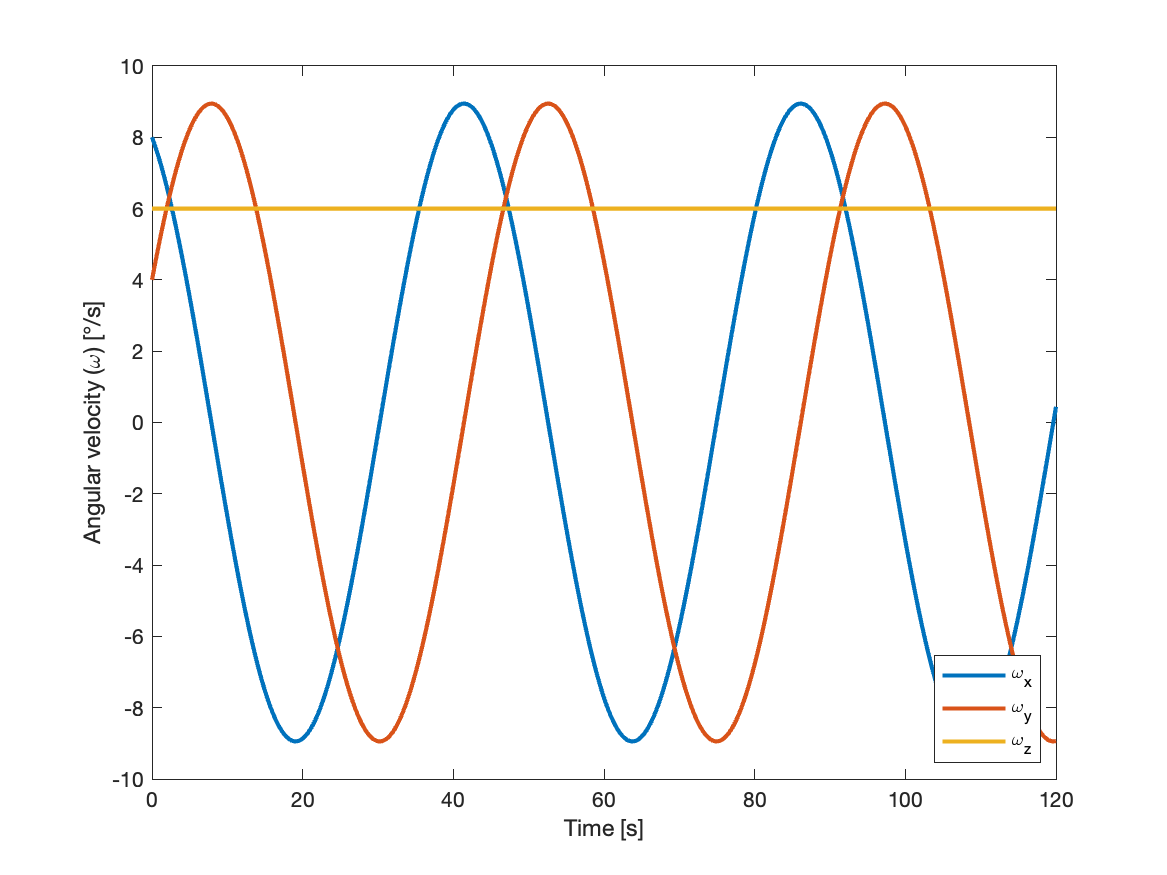
\includegraphics[scale=0.6]{Images/ps3_problem1.png}
\caption{Numerical solution results}
\label{fig:ps3_problem1}
\end{figure}


\subsection{PROBLEM 2}
\textit{Program analytical solution for axial-symmetric satellite. Compute it at same time steps and from same initial conditions.}

\begin{figure}[H]
\centering
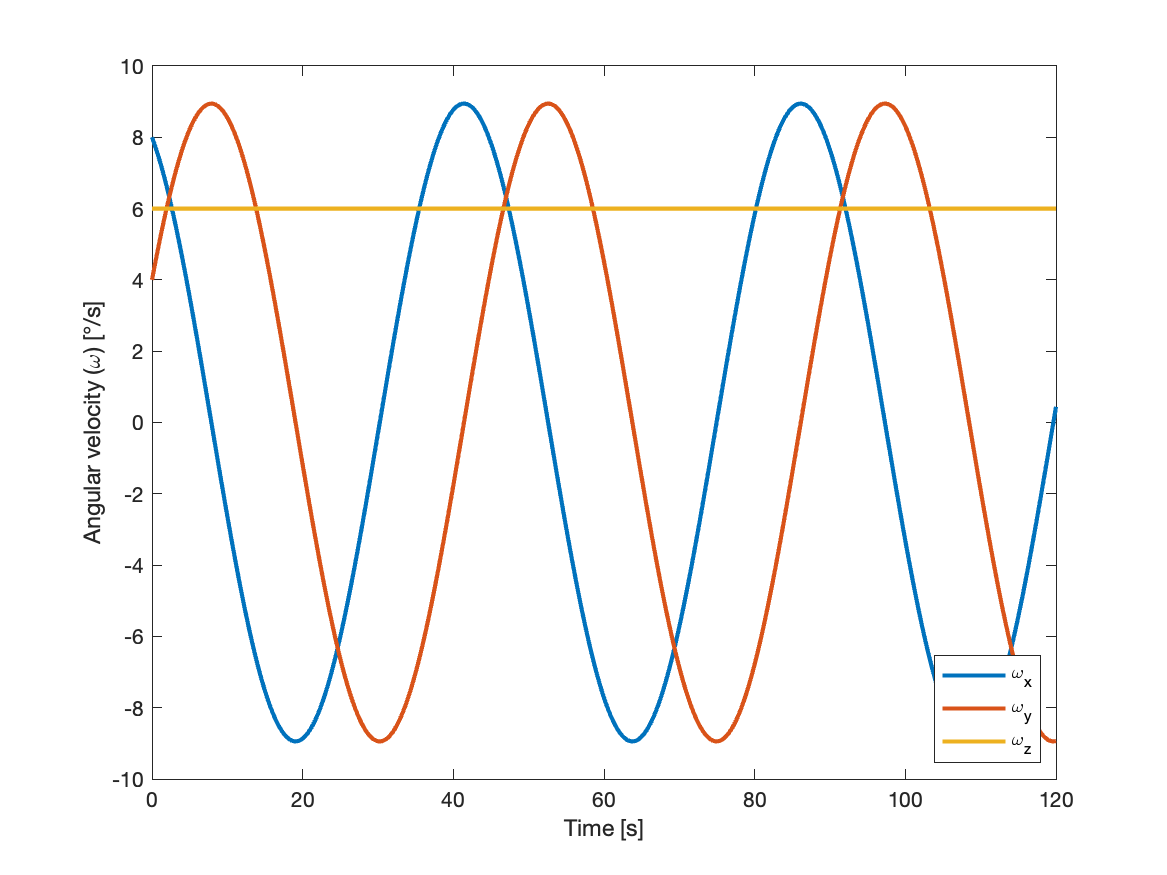
\includegraphics[scale=0.6]{Images/ps3_problem2.png}
\caption{Analytical solution results}
\label{fig:ps3_problem2}
\end{figure}


\subsection{PROBLEM 3}
\textit{Compare numerical and analytical solutions. Plot differences (errors), do not only superimpose absolute values. Tune numerical integrator for large discrepancies. Are angular velocity vector and angular momentum vector changing according to theory in principal axes?}

\begin{figure}[H]
\centering
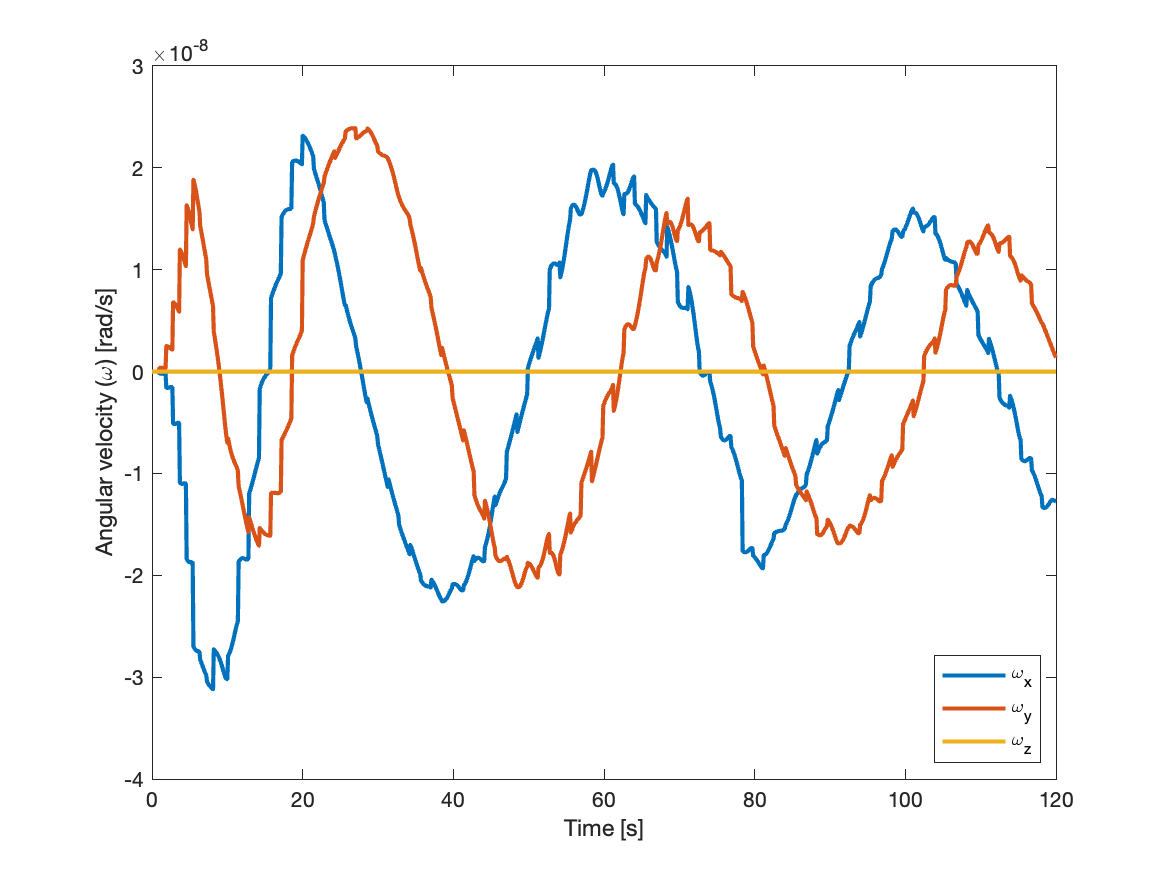
\includegraphics[scale=0.6]{Images/ps3_problem3.png}
\caption{Error between numerical and analytical solutions}
\label{fig:ps3_problem3}
\end{figure}


\subsection{PROBLEM 4}
\textit{Program Kinematic equations of motion correspondent to a nominal attitude parameterization of your choice.}

We choose a nominal attitude parameterization of quaternions, our choice being based on the absence of singularities. The following function computes the time derivative for a state consisting of quaternions (4 parameters) and angular velocity (3 parameters).

\lstinputlisting{src/kinQuaternion.m}

We can use the previous function to perform a forward Euler numerical integration. We call the previous function over a fixed time step to compute the evolution of the state.

\lstinputlisting{src/kinQuaternionForwardEuler.m}

For improved precision, we implement a 4th order Runge-Kutta method, which uses a weighted sum of slopes to obtain a better result. This also calls the time derivative function, but does so with different values of the state, which are weighted to obtain the next state for each step.

\lstinputlisting{src/kinQuaternionRK4.m}


\subsection{PROBLEM 5}
\textit{Program Kinematic equations of motion correspondent to a different attitude parameterization from the previous step. This is used for comparison, to get familiar with different approaches, and as fall back solution in the case of singularities.}

Similarly, we create a function which computes the time derivative of a state consisting of Euler angles and angular velocity.

\lstinputlisting{src/kinEulerAngle.m}

We can propagate this with forward Euler, as in the previous section.

\lstinputlisting{src/kinEulerAngleForwardEuler.m}

For our actual implementation, we choose to use the time derivative function with \texttt{ode113} for improved accuracy. Note that while this is possible with the Euler angle time derivative, it cannot be done as simply for quaternions, as they require normalization at each step, hence our decision to implement RK4.


\subsection{PROBLEM 6}
\textit{Numerically integrate Euler AND Kinematic equations from arbitrary initial conditions (warning: stay far from singularity of adopted parameterization). Multiple revolutions. The output is the evolution of the attitude parameters over time. These attitude parameters describe orientation of principal axes relative to inertial axes.}


\subsection{PROBLEM 7}
\textit{Since inertial position, velocity, and attitude, are known at the same time throughout the simulation, it is now possible to express vectors in the reference systems of interest.}

